\chapter{Sample Chapter} \label{ch:sample}

%============================= INTRODUCTION =================================
\section{Introduction}\label{sec:i}
Remember that wherever you want you can cite with \verb.\cite{a1}. \cite{DBLP:journals/ieeemm/BalduiniVALAC15} someone.
Or use \verb.\footnote{That's a footnote}. like this\footnote{That's a footnote} 
% this is used to include other .tex files in order to split a long document 

%============================= SECTIONS =================================

\section{New section}
You can insert a definition
	\begin{Definition}
		PoliMi: Politecnico di Milano
	\end{Definition}
	
\section{Another section}
	\subsection{And a subsection}
		In this sub section I will include many images just to make the list of figures meaningful.

			\begin{figure}[h!tb]
				\centerline {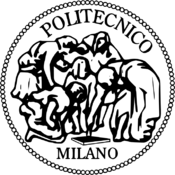
\includegraphics[scale=0.6]{img/logopoli.png}}
				\caption{Caption of this PoliMi image.}
				\label{fig:leet}
			\end{figure}

\section{New section}
	\subsection{And also many sub}
		\subsubsection{Or again more nested}
			\begin{itemize}
				\item item 1
				\item item 2
				\item item 3
			\end{itemize}			
			
\section{New section}
This is an example of table. You can see it in Table~\ref{tab:TableName}. 

 \begin{table}[h!tb]
   \centering \caption{Table caption}
   \label{tab:TableName}
   \vskip 0.2cm
   %%
   \scalebox{0.90}{
	    %% The {|c|c|c|c|c|} define the number of columns.
	    %% c means centered
	    %% | defines a vertical line between two columns 
	    \begin{tabular}{|c|c|c|}
	      \hline
	      Col 1 & Col 2 & Col2  \\
	      %% \\ force a newline without creating an horizontal line
	      Dim C.1 & Dim C.3 & Dim C.3 \\
	      %% \hline create an horizontal line between two rows
	      \hline
	      Data 1.1 & Data 1.2 & Data 1.3 \\
	      \hline
	      Data 2.1 & Data 2.2 & Data 2.3 \\
	      \hline
	      Data 3.1 & Data 3.2 & Data 3.3 \\  
	      \hline
	    \end{tabular}
	 }
 \end{table}

\section{You can do as many section as you want}
The following equation has been created using \verb.$$.: $ y_1 = a*x + b$.

%% \smallskip introduces a small vertical skip
\smallskip

%% \noindent is used to eliminate the blankline and the paragraph settings 
\noindent
This is a more complex equation: \[ y_2 = a*x + b \], created using \verb.\[ \].

%% \bigskip introduces a big vertical skip
\bigskip

\noindent
This is, (\ref{eq:eeq1}), an enumerated equation: 

	\begin{equation}\label{eq:eeq1}
		y_3 = a*x + b
	\end{equation}

, created using:

	\begin{verbatim}
		\begin{equation}\label{eq:eeq1}
		    y_3 = a*x + b
		\end{equation}
	\end{verbatim}


